In this paper we propose an interactive workflow and a visual user interface to help data scientists and domain experts diagnose and validate binary classifiers. The approach we suggest is based on a mix of automated and interactive methods that guide the user towards understanding what decisions a model makes, which ones are correct or incorrect, and potential strategies to improve them.

Being able to explore the decisions a model makes and identifying potential issues is crucial in application areas where experts need to get a sense of how the model works and build trust in its decisions. While common practice in much of the machine learning endeavors is to focus on model accuracy, many researchers have voiced the need for more transparency when the application domain requires it~\cite{baesens2003using, Caruana:2015:IMH:2783258.2788613, freitas2014comprehensible, lou2012intelligible, martens2007comprehensible, vellido2012making}. A recent DARPA (Defense Advanced Research Projects Agency) program called ``Explainable AI (XAI)", for example, calls for more research in this area and declares, as the main motivation for the program that ``\textit{the effectiveness of these systems is limited by the machine’s current inability to explain their decisions and actions to human users}" and that ``\textit{it is essential to understand, appropriately trust, and effectively manage an emerging generation of artificially intelligent machine partners}".

In addition to evaluating a model in terms of accuracy, we propose the idea of \textit{semantic validation}, the need for domain experts to verify that the decisions a model makes are plausible when compared against their mental models of the problem. For instance, in healthcare settings, medical doctors often want to see examples of recommendations the model provides and need to gain trust in it before they feel comfortable with deploying it in real-world settings.
Such reservations in deploying models without having an opportunity to manually verify what decisions they make are well justified as it is entirely possible for a model to achieve high accuracy and yet provide dramatically erroneous recommendations~\cite{Caruana:2015:IMH:2783258.2788613}.

Another important factor to consider is that domain experts and data scientists are often working in collaboration to solve a particular problem (or they are actually the same person covering both roles). Being able to manually inspect a model can give them an opportunity to generate useful insights on how a model can be improved. While commonly used aggregate statistics such as area under the curve (AUC) give a sense of the overall accuracy of the model, and can be used as a parameter to compare between different models, they do not provide insights on how or why a model fails to capture important phenomena accurately.

Some existing methods do provide more transparency and useful information for enabling better understanding and diagnostic purposes, but they tend to be limited and specific to a particular kind of model. For example, \textit{logistic regression} and \textit{decisions trees} are commonly regarded as more interpretable models thanks to their ability to provide information on feature weights and / or specific decisions the model makes (decision trees)~\cite{freitas2014comprehensible}. These solutions are however limited by a number of factors. Since they are specific to the selected method, they are hard to generalize and cannot be applied transparently to other types of models. Furthermore, they only provide a limited picture of what decisions the model makes. Feature weights provide a highly coarse summary of how relevant features are \textit{globally}, but they do not provide information on how the model makes decisions \textit{locally}, for a selected set of instances. Even more transparent methods, like decision trees, tend to grow very large and are not easy to parse visually, especially for data sets with a high number of dimensions / features.

\begin{figure}[t]
\centering
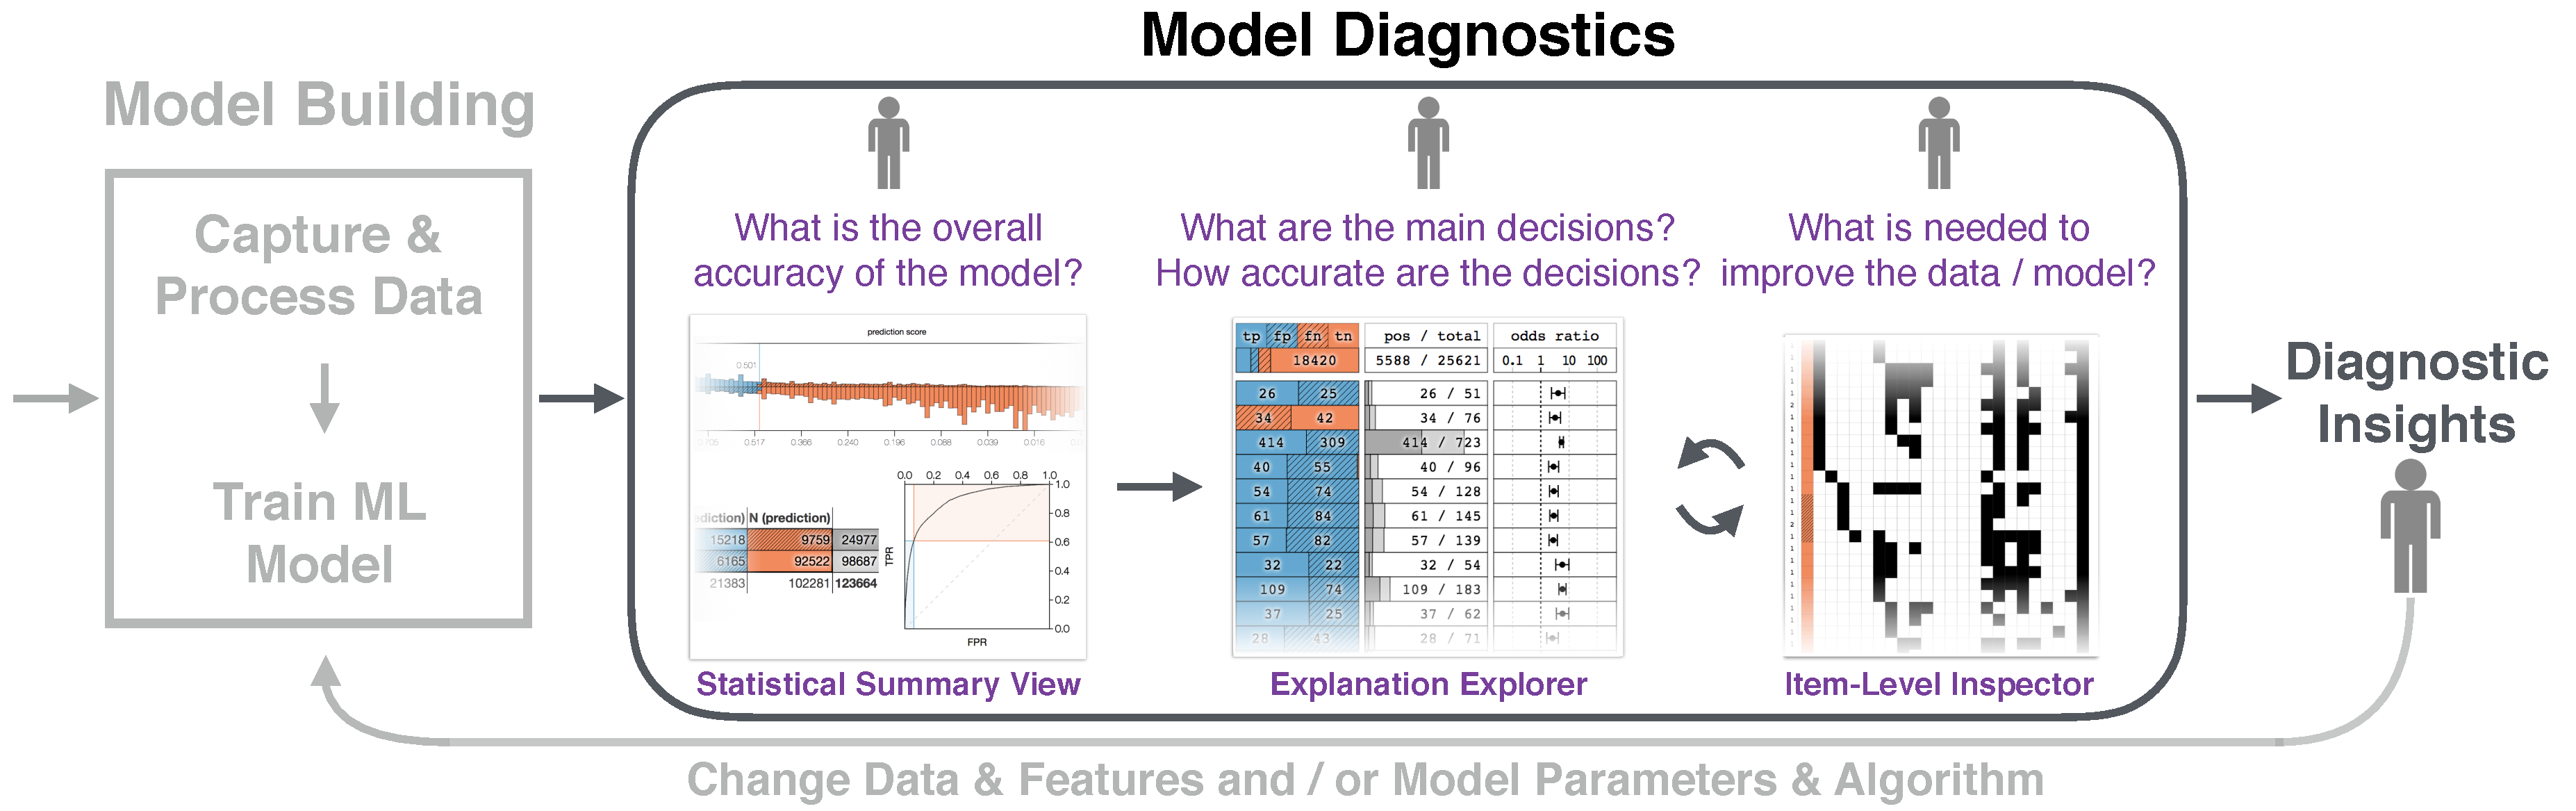
\includegraphics[width=\textwidth]{explainer/workflow5}
\caption[The Model Diagnostics workflow.]{
Our proposed \textbf{Model Diagnostics} workflow extends the conventional \textit{Model Building} workflow in machine learning for enabling domain experts to reason about the semantic validity of the decisions made by any model through multiple linked visualizations of statistical performance summaries, explanations, and item-level distribution of features. By iterating through explanation-level summaries and item-level details, experts are able to generate diagnostic insights about the quality of both the data and the model. This ultimately helps to improve data acquisition and model generation processes belonging to the original workflow.
}
\label{figs:workflow}
\end{figure}

% An explanation comprises of a set of features that need to be removed to change the label for a given item. 

To address these issues we propose a workflow, aimed at machine learning experts and data scientists, based on \textit{instance-level explanations}, computational methods to derive a description of how a model makes decisions on single data items, without having access to the internal logic of the model (\ie, using the model as a \textit{black box}). These explanations are then aggregated and used as input to a visualization system that enables the browsing of model decisions and assessment of their quality.

The work we describe in the paper stems from a one year collaboration with a group of domain and machine learning experts~from the \textit{NYU Langone Medical Center}.
%~({two of them are co-authors of this paper})
In our collaboration, we worked together to make sense of models built to understand how patients are handled in the hospital and to figure out whether important outcomes of interest can be predicted correctly. This resulted in the development of an interactive model diagnostic workflow using visual explanations of model behavior that is the main contribution of this work.
% main outcome of this interaction is the workflow and interfaces we describe in the paper
% \aritra{I feel this paragraph about section organizations is not needed.}
The rest of the paper is organized as follows. We present related work in the next section. We provide an overview of model diagnostics goals and of the proposed workflow in Section~\ref{sec:model-diagnostics}. We then describe in detail the instance-level explanation algorithm we use in Section~\ref{sec:algo} and the interfaces we built in Section~\ref{sec:ui}. Section~\ref{sec:case_study} reports on a use case we built to show how the workflow can help perform useful and actionable model diagnostics. Section~\ref{sec:discussion} discusses the results and provides a number of reflections and lessons we have learned from this collaborative exercise.

%In our work, we use a method developed by Marteens et al.~\cite{}, which works on binary classification with sparse high-dimensional data set and creates explanations in form of the set of features the model uses to make a decision on a single instance.



% ---
% when using predictive modeling as part of their analysis workflow, are frequently confronted with questions as: ``Do the model predictions make sense?", ``Can I trust this model?" To answer these questions, merely optimizing the model performance for achieving the best match between predicted and actual outcomes is not sufficient. Statistical performance measures can indicate correctness, but they do not ensure that the model is actually plausible and can be trusted.

% While a very large proportion of the efforts in predictive modeling is on achieving accurate \textit{predictions}, little has been done to systematically assure that a model is able to provide plausible \textit{explanations} of the intricate set of relationships between features, their values, and the outcome. To fill this gap, we propose a diagnostic workflow that can enable both data scientists and non-machine learning domain experts in \textit{semantic validation} of binary classifiers by observing input-output relationships of models through the lens of visual explanations.

% We derive this workflow through a long-standing collaboration with doctors and healthcare experts. In healthcare settings it is crucial to derive insights on \textit{why} and \textit{how} a model relates a set of patient descriptors (patient history) to a given medical outcome of interest (disease onset). In this scenario, global explanations of model behavior are not sufficient: experts often need to focus on subsets of patients or a single patient, find features related to the predicted label, verify if they are meaningful, and accordingly get insight into both global and local predictions of the classifier. To address this, at the core of our workflow are instance-level visual explanations: explanations that are based on measures of local feature relevance for single instances in the data. These are communicated through visual representations that help guide the experts in diagnosing why and how a classifier makes its decisions.

% In our approach, we treat a classifier as a black-box. This has two advantages. First, the approach can be generalized for any existing classification model. Second, without having to access its internal structure, data scientists and domain experts alike can observe the input / output behavior of a model and diagnose model decisions for developing trust in them.

% In the rest of the paper we first investigate related work and describe the motivation and design decisions for the diagnostic workflow. Second, we focus on the description of the visual interface by mapping the domain experts' tasks to the different visual representations and interactions. Next, we describe two use cases derived from our collaboration that validate the efficacy of our workflow. We also reflect on the generalizable lessons learnt about how visual explanations can be used to inspire trust in domain experts about the semantic validity of model predictions.







% Requires semantic validation, going beyond statistical measures of model performance. drawbacks: lack of generalizability, most applications for model tuning.

% We derive a workflow, healthcare, model diagnsotics. data scientists: features that are necessary, domain experts, incorporate their domain knowledge


% \begin{itemize}
%     \item \joschi{TODO -- commented old introduction which doesn't focus on explanations for debugging though}
% \end{itemize}
% \joschi{rewrite}
% In this paper we use visual analytics to discover and explore explanations of decisions made by a binary classifier. \joschi{TODO: too vague}

% Many real-world scenarios require analysts to understand how a set of many independent features and a target of interest relate to each other; that is, which combinations of features and values lead to a given outcome. For example, this includes: how words used in product reviews relate to the number of stars assigned by reviewers or how physiological measures and medications affect patient admission in a hospital.

% Predictive modeling using classification techniques is a very common approach to solve those kind of problems as classification methods are meant to build models that capture associations between values and a target. Experts usually optimize those models for achieving the best match of predicted and actual outcomes. While this is necessary for predictive modeling to work correctly it does not ensure that the model is actually plausible and to be trusted.

% \joschi{example of a situation -- pneumonia/astma example of \url{http://people.dbmi.columbia.edu/noemie/papers/15kdd.pdf}}

% For instance, in healthcare settings it is crucial to derive insights on \textit{why} and \textit{how} a model relates a set of patient descriptors (patient history) to a given medical outcome of interest (disease onset) in order to be actually useful in practice and trusted by doctors. Even if the prediction of the model is always correct on the test data set; without confirming the correctness of the decision \textit{making} process the correctness of the model cannot be guaranteed in general.

% While a very large proportion of the efforts in predictive modeling is on achieving accurate \textit{predictions}, little has been done to systematically assure that a model is able to provide plausible \textit{explanations} of the intricate set of relationships between features, their values, and the outcome.

% \joschi{what are you actually proposing here?}
% A common approach of giving insights into the decision making
% process of a machine learning model is to assign importance
% to features in the data set.
% This is usually done globally without regard for individual nuances (\joschi{TODO: cite some papers maybe?}).
% Thus, this does not provide insights into actual decisions
% being made but rather how influential certain features
% are in general.

% A more sophisticated approach that is gaining more popularity
% recently \cite{prospector,Martens:2014:EDD:2600518.2600523,DBLP:journals/corr/RibeiroSG16} is to locally assign feature importance to individual items.
% This is achieved by generating hypothetical inputs to the machine learning model to examine how an observed data point needs to be changed in order to \textit{change} the predicted outcome.
% This gives insight into which features are responsible for the original prediction of the observed data point.
% The set of locally important features is thus called the ``explanation" of a data point.

% This approach generates individual explanations for every observed
% item in the data set.
% Using aggregation and visual analytics helps coping with this vast amount of additional meta data enabling domain experts to analyze the correctness of the decision making process on a population level rather than on a case-by-case basis.

% \joschi{TODO: give teaser of the VA interface -- HOW still missing}

% Our contributions are concretely:
% \begin{itemize}
%     \item Tasks needed to check plausibility of and gain trust in decisions made by a machine learning model.
%     \item A rich visual analytics application aimed at solving those tasks.
% \end{itemize}

% \joschi{TODO: paper structure}
